\chapter{Load Balancing Tool and Detailed Program
  Description}\label{lbdetails}
A \textbf{load balancer} is a tool that dynamically reassigns tasks as the
processors complete their work. There are many strategies for load
balancing, such as sender initiated diffusion, receiver initiated
diffusion, hierarchical balance model, etc.~\cite{dlb}. The Load
Balance tool on Janus uses a master-slave strategy for
balancing~\cite{janus}. In general, a load balancer recognizes the
number of processors that are going to be used in a simulation, and manages
the workload distribution among
them. Figure~\ref{fig:loadbalance_overall} demonstrates the load
balancer coordinating tasks over three nodes. 
\begin{figure}[htp]
\caption[Load balancing example]{Load balancing example over
  three nodes. The load balancer is invoked over 3 nodes; it determins
the work distribution over each node.}\label{fig:loadbalance_overall}
	\begin{center}
          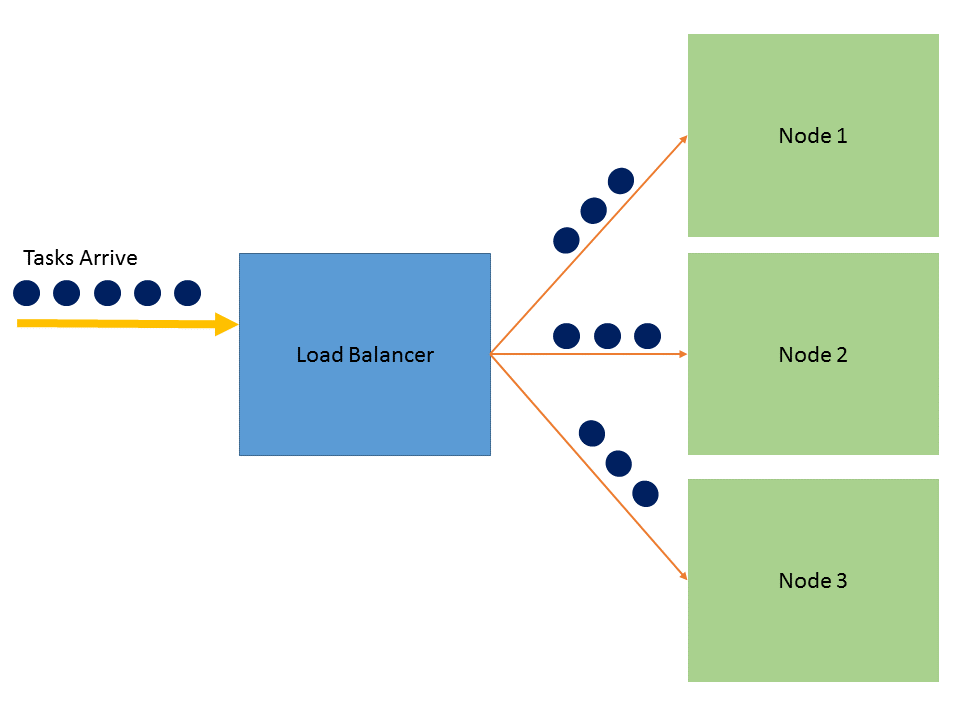
\includegraphics[scale=0.35]{figs/loadbalance_overall.png}
	\end{center}
\end{figure}
If, for example, Processor A finishes its load early
(perhaps its initial condition led to near-immediate convergence),
the load balancer assigns Processor A more work by reducing the
queue of tasks on Processor B (a processor taking more time to complete its
current task) and passing some tasks to Processor A. Figure~\ref{fig:loadbalance_node}
shows how the load balancer reassigns tasks between the 12 processors
on any given node.
\begin{figure}[htp]
\caption[Processor work distribution before and after load
balancing]{As tasks arrive, each processor in a node takes an initial
  task (left). As the processors finish their task, the ones who finish first are
assigned more work while the others continue running (right).}\label{fig:loadbalance_node}
\centering
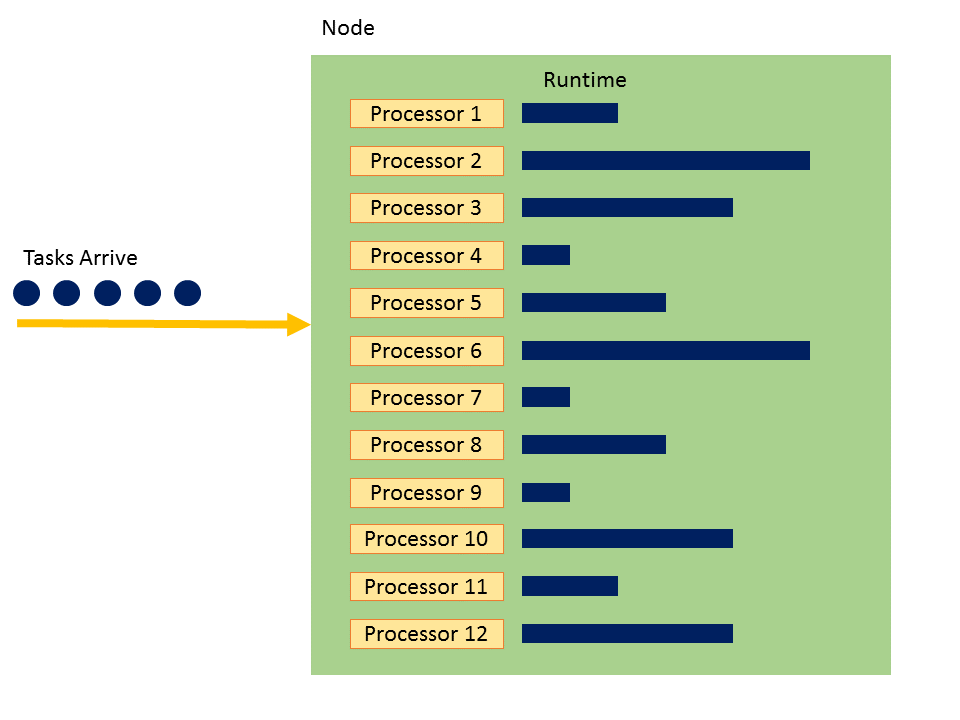
\includegraphics[width=.5\textwidth]{figs/loadbalance_node_start.png}\hfill
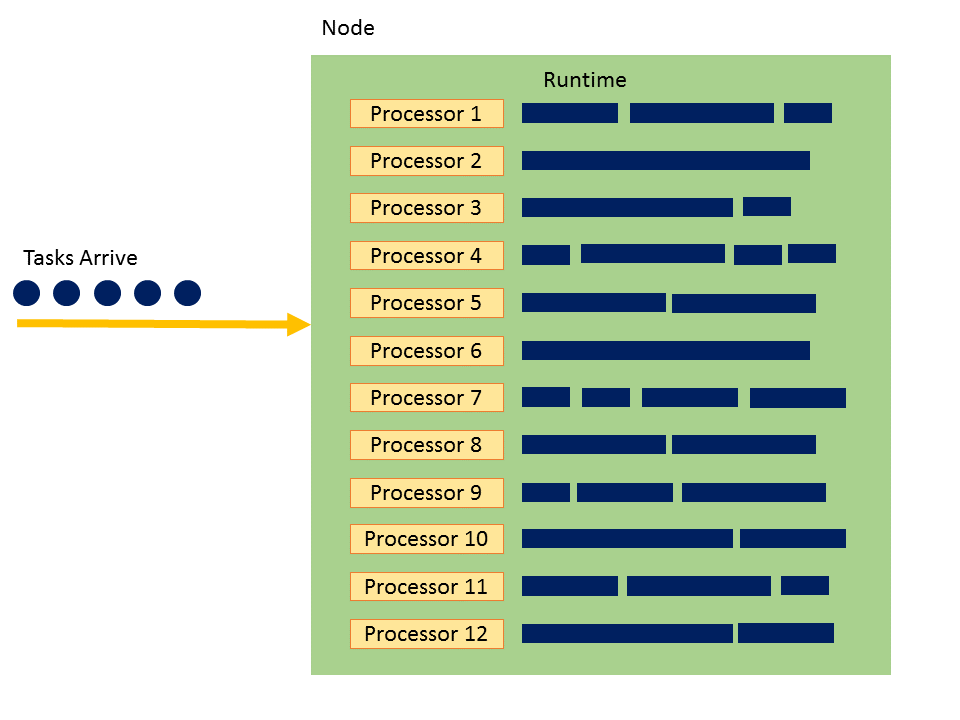
\includegraphics[width=.5\textwidth]{figs/loadbalance_node_end.png}
\end{figure}
Figure~\ref{fig:lbtool} demonstrates an example of a simulation
using 40 nodes on Janus, where there are 12 processors per
node. Below is an outline of how each processor is called in the program. 
\begin{enumerate}
\item Each processor should take a different initial $x_0$ and report
  whether the initial condition led to finding a stable orbit  
\begin{itemize}
\item The load balancer determines work distribution over the processors.
\end{itemize}
\item Repeat the above steps for a large number of different random
  maps $R_i(x)$, $i = 0, 1, 2,... \bar{N}$ in order to find the sample
  mean of any given order $p$ periodic orbit and the orbit locations
  (if there was convergence).
\begin{itemize}
\item Use the data to produce a histogram of periodic orbits that depicts the expected number of order $p$ periodic orbits for the random map
\item Create bifurcation diagrams for various values of $L$.
\item Use a HDF5 file to store the simulation data
\end{itemize}
\end{enumerate}

\begin{figure}[htp]
\caption[Load balancing tool overview]{Load Balancing Tool Overview:
  The load balancer is invoked over 40 nodes, where each node handles
  some value of $r \in [0,4]$ and a number $N_x$ of initial conditions
  $x_0 \in [0,1]$ are tested. Each node produces a datafile, which is
  compiled with the other results to create a bifurcation diagram or
  histogram of periodic orbits.}\label{fig:lbtool}
	\begin{center}
          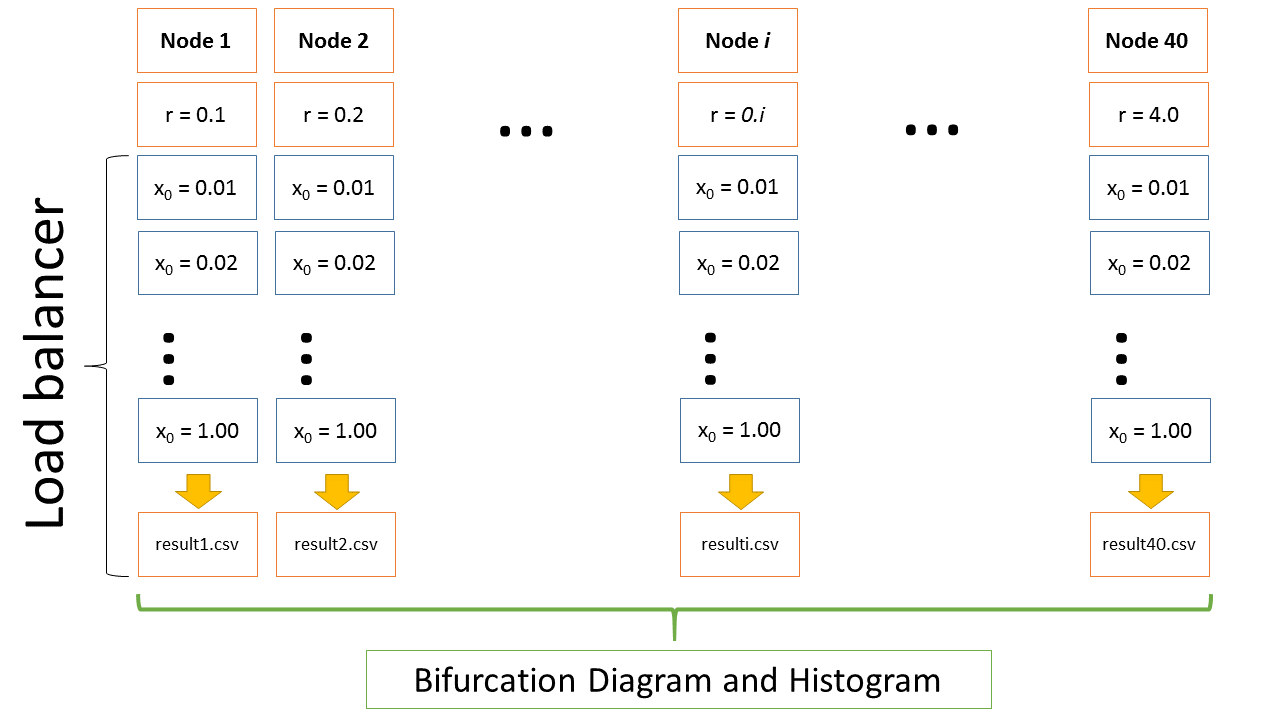
\includegraphics[scale=0.45]{figs/load_balancer.png}
	\end{center}
\end{figure}

The original simulation was written in serial code in
MATLAB, and had extremely variable runtimes (due to the nature of fixed
point iteration). The original version of the code was rewritten for efficiency,
speed, and scalability. The new implementation, written in C++ and
Python, was capable of reproducing two types plots: histograms of observed periodic
orbits and bifurcation diagrams for varying values of the correlation
length, $L$. Figure~\ref{fig:workflow} is a workflow of the
program structure, and we offer a detailed program description below.

The program begins with \texttt{generate\_cmdlines}, where the user
specifies the desired parameters for the simulation. The resulting
data may be processed and visualized as a histogram of periodic orbits
or bifurcation
diagram. 
\begin{enumerate}
\item \texttt{generate\_cmdlines}: the set up file for the simulation;
specifies the parameters used in the map realizations. It will
generate all the bash script files needed by Janus's work scheduler, \texttt{slurm}.
\item bash scripts: Each of these scripts will invoke
  \texttt{generate\_rands}, based on parameters given in
  \texttt{generate\_cmdlines}. \texttt{generate\_rands} creates a data
  file of values of $a_n,b_n$, the Fourier modes of $\xi(x)$. The
  script \texttt{myfunc} uses the output from
  \texttt{generate\_rands}.
\item \texttt{generate\_rands}: Generate randomized parameters $a_n,b_n$
  and write them to file for the parameters specified by \texttt{generate\_cmdlines}.
\item \texttt{myfunc}: Iteratively solve the map $f(x) = x$, and print out
  the orbit locations if they exist or return nothing if the map
  diverges. All output from \texttt{myfunc} will be fed into a
  \texttt{result} file associated with the given bash script. 
\item \texttt{csv2hdf5}: Convert \texttt{result} to a HDF5 file
  while checking for uniqueness in the data
  set. Save the processed data in an HDF5 file for archival
  purposes. 
\item \texttt{unique}: Check for uniqueness in the data set and create a histogram of the data
\item \texttt{plotbif}: Use the HDF5 file to produce the bifurcation diagram. 
\end{enumerate}
 
\begin{figure}[htp]
\caption[Load balancing workflow]{Load Balancing Workflow: The load
  balancing tool on Janus takes as input a list of commandline prompts
  (created by \texttt{generate\_cmdline}) calling the
  executable files \texttt{myfunc} and
  \texttt{generate\_rands}. \texttt{generate\_cmdline}
  specifies the parameters the user intends to test for the
  simulation. Each node produces a file called \texttt{result},
  which is parsed by \texttt{Unique} and \texttt{csv2hdf5} to get
  a set of unique orbits to store in a HDF5 file. \texttt{Unique} also creates the histogram. The final script, \texttt{plotbif}, generates the bifurcation diagram.}\label{fig:workflow}
	\begin{center}
          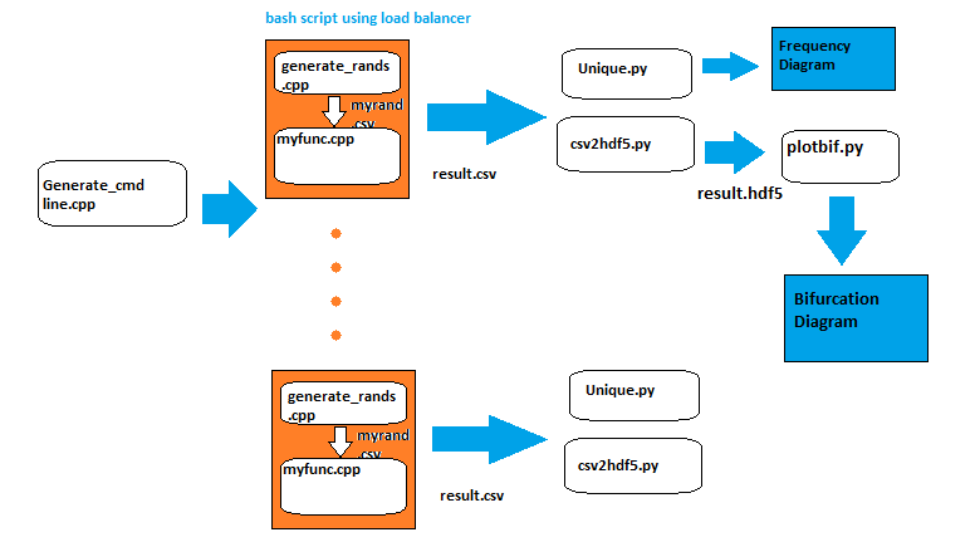
\includegraphics[scale=0.5]{figs/workflow.png}
	\end{center}
\end{figure}

The HDF5 file format was used to store the simulation results in a better
archival format. Single core optimization techniques, such as SIMD loop
vectorization and function inlining, as well as using a dynamic load
balancer for more efficient work distribution were
applied. The following are the optimization techniques applied:
\begin{itemize}
\item Preferential use of the multiply and add operators where possible, since
they are less expensive than divide and subtract operators
\item Used a reduction on the loop that computes the Fourier Series
  in order to take advantage of the data parallelism with SIMD
\item Loop structure was reorganized to take advantage of C++ being
  row-oriented (outer loop should go by rows, then inner loops go by columns)
\item Functional inlining in the C++ code to reduce the number of function calls
\item The lack of a built in uniform random number generator that generates a random
double between two doubles led to the creation of a pseudo random number
generator with the use of \texttt{rand} and \texttt{srand}.
\end{itemize}

The benchmarking (strong scaling study) results (Figure~\ref{fig:effsp}) imply
the best speedup and efficiency is gained when invoking the load balancer on
one node (12 processors), although we tested our simulation over 16 nodes
(192 processors). The formulas for calculating speedup $S$ and
efficiency $E$ are
\begin{align}
\begin{split}
S &= \frac{t_s}{t_l}\\
E &= \frac{S}{n_p},
\end{split}
\end{align}
where $t_s$ is the serial computation time, $t_l$ is the load balanced
computation time, and $n_p$ is the number of processors used. However,
since the original serial implementation in MATLAB could take days to complete,
the speedup and efficiency in Figure~\ref{fig:effsp} was computed using a
serial implementation in C++, so these plots reflect speedup and
efficiency where single core optimization has already been applied. The
diminishing speedup and efficiency for larger numbers of processors is
likely due to the overhead cost of coordinating tasks over many
processors and nodes. 
\begin{figure}[htp]
\caption[Impact of the load balancing tool: efficiency and
speedup]{Efficiency (left) and Speedup (right) of the new
  implementation. The best efficiency occurred for one node, and the best speedup was also achieved for 1 node.}\label{fig:effsp}
\centering
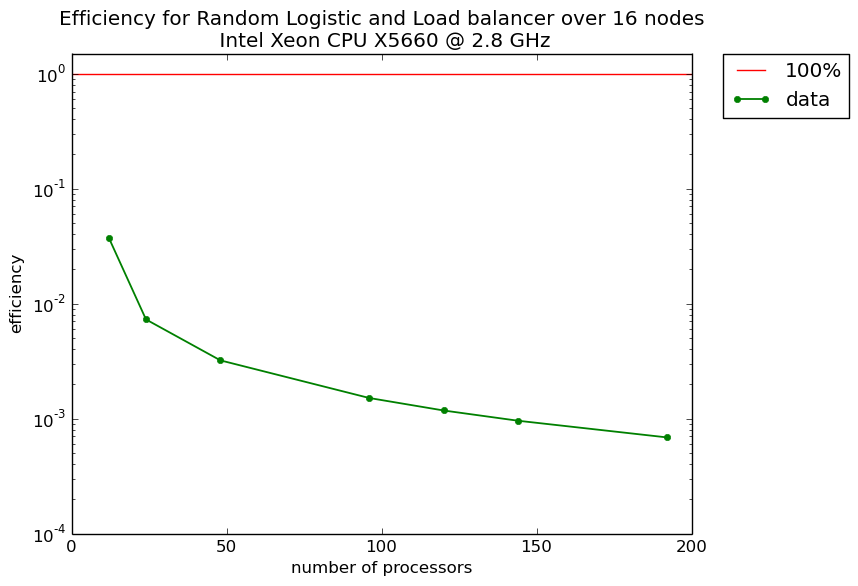
\includegraphics[width=.5\textwidth]{figs/efficiency_random_logistic.png}\hfill
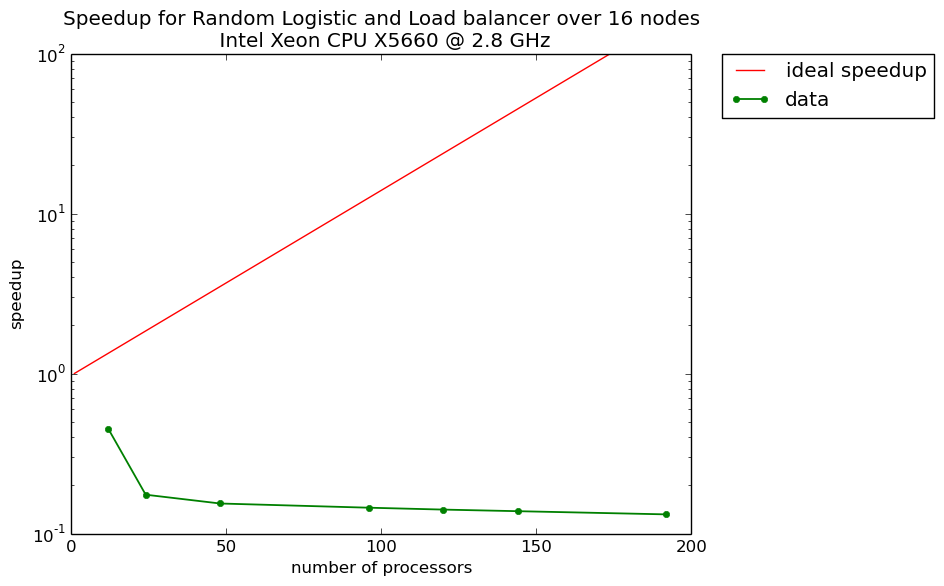
\includegraphics[width=.5\textwidth]{figs/speedup_random_logistic.png}
\end{figure}

